%%%%%%%%%%%%%%%%%%%%%%%%%%%%%%%%%%%%%%%%%
% Beamer Presentation
% LaTeX Template
% Version 2.0 (March 8, 2022)
%
% This template originates from:
% https://www.LaTeXTemplates.com
%
% Author:
% Vel (vel@latextemplates.com)
%
% License:
% CC BY-NC-SA 4.0 (https://creativecommons.org/licenses/by-nc-sa/4.0/)
%
%%%%%%%%%%%%%%%%%%%%%%%%%%%%%%%%%%%%%%%%%

%%%%%%%%%%%%%%%%%%%%%%%%%%%%%%%%%%%%%%%%%
% This presentation template is an adaptation of the template mentioned above. It has been created by Giovanni Spadaro and it is available on GitHub (https://github.com/Giovo17/presentation-template-unict-lm-data).
%%%%%%%%%%%%%%%%%%%%%%%%%%%%%%%%%%%%%%%%%

%----------------------------------------------------------------------------------------
%	PACKAGES AND OTHER DOCUMENT CONFIGURATIONS
%----------------------------------------------------------------------------------------

\documentclass[
	11pt, % Set the default font size, options include: 8pt, 9pt, 10pt, 11pt, 12pt, 14pt, 17pt, 20pt
	%t, % Uncomment to vertically align all slide content to the top of the slide, rather than the default centered
	%aspectratio=169, % Uncomment to set the aspect ratio to a 16:9 ratio which matches the aspect ratio of 1080p and 4K screens and projectors
]{beamer}

\graphicspath{{img/}} % Specifies where to look for included images (trailing slash required)

\usepackage{booktabs} % Allows the use of \toprule, \midrule and \bottomrule for better rules in tables

%----------------------------------------------------------------------------------------
%	SELECT LAYOUT THEME
%----------------------------------------------------------------------------------------

% Beamer comes with a number of default layout themes which change the colors and layouts of slides. Below is a list of all themes available, uncomment each in turn to see what they look like.

%\usetheme{default}
%\usetheme{AnnArbor}
%\usetheme{Antibes}
%\usetheme{Bergen}
%\usetheme{Berkeley}
%\usetheme{Berlin}
\usetheme{Boadilla}
%\usetheme{CambridgeUS}
%\usetheme{Copenhagen}
%\usetheme{Darmstadt}
%\usetheme{Dresden}
%\usetheme{Frankfurt}
%\usetheme{Goettingen}
%\usetheme{Hannover}
%\usetheme{Ilmenau}
%\usetheme{JuanLesPins}
%\usetheme{Luebeck}
%\usetheme{Madrid}
%\usetheme{Malmoe}
%\usetheme{Marburg}
%\usetheme{Montpellier}
%\usetheme{PaloAlto}
%\usetheme{Pittsburgh}
%\usetheme{Rochester}
%\usetheme{Singapore}
%\usetheme{Szeged}
%\usetheme{Warsaw}

%----------------------------------------------------------------------------------------
%	SELECT COLOR THEME
%----------------------------------------------------------------------------------------

% Beamer comes with a number of color themes that can be applied to any layout theme to change its colors. Uncomment each of these in turn to see how they change the colors of your selected layout theme.

%\usecolortheme{albatross}
%\usecolortheme{beaver}   % red
%\usecolortheme{beetle}
%\usecolortheme{crane}   % yellow
%\usecolortheme{dolphin}  % purple
%\usecolortheme{dove}   % white
%\usecolortheme{fly}   % grey
%\usecolortheme{lily}   % purple
%\usecolortheme{monarca}   % yellow background and black
%\usecolortheme{seagull}
%\usecolortheme{seahorse}
%\usecolortheme{spruce}   % green
\usecolortheme{whale}
%\usecolortheme{wolverine}

%----------------------------------------------------------------------------------------
%	SELECT FONT THEME & FONTS
%----------------------------------------------------------------------------------------

% Beamer comes with several font themes to easily change the fonts used in various parts of the presentation. Review the comments beside each one to decide if you would like to use it. Note that additional options can be specified for several of these font themes, consult the beamer documentation for more information.

\usefonttheme{default} % Typeset using the default sans serif font
%\usefonttheme{serif} % Typeset using the default serif font (make sure a sans font isn't being set as the default font if you use this option!)
%\usefonttheme{structurebold} % Typeset important structure text (titles, headlines, footlines, sidebar, etc) in bold
%\usefonttheme{structureitalicserif} % Typeset important structure text (titles, headlines, footlines, sidebar, etc) in italic serif
%\usefonttheme{structuresmallcapsserif} % Typeset important structure text (titles, headlines, footlines, sidebar, etc) in small caps serif

%------------------------------------------------

%\usepackage{mathptmx} % Use the Times font for serif text
\usepackage{palatino} % Use the Palatino font for serif text

%\usepackage{helvet} % Use the Helvetica font for sans serif text
\usepackage[default]{opensans} % Use the Open Sans font for sans serif text
%\usepackage[default]{FiraSans} % Use the Fira Sans font for sans serif text
%\usepackage[default]{lato} % Use the Lato font for sans serif text

%----------------------------------------------------------------------------------------
%	SELECT INNER THEME
%----------------------------------------------------------------------------------------

% Inner themes change the styling of internal slide elements, for example: bullet points, blocks, bibliography entries, title pages, theorems, etc. Uncomment each theme in turn to see what changes it makes to your presentation.

%\useinnertheme{default}
\useinnertheme{circles}
%\useinnertheme{rectangles}
%\useinnertheme{rounded}
%\useinnertheme{inmargin}

%----------------------------------------------------------------------------------------
%	SELECT OUTER THEME
%----------------------------------------------------------------------------------------

% Outer themes change the overall layout of slides, such as: header and footer lines, sidebars and slide titles. Uncomment each theme in turn to see what changes it makes to your presentation.

\useoutertheme{default}
%\useoutertheme{infolines}
% \useoutertheme{miniframes}
% \useoutertheme{smoothbars}
%\useoutertheme{sidebar}
%\useoutertheme{split}
%\useoutertheme{shadow}
%\useoutertheme{tree}
%\useoutertheme{smoothtree}

%\setbeamertemplate{footline} % Uncomment this line to remove the footer line in all slides
%\setbeamertemplate{footline}[page number] % Uncomment this line to replace the footer line in all slides with a simple slide count

%\setbeamertemplate{navigation symbols}{} % Uncomment this line to remove the navigation symbols from the bottom of all slides

%----------------------------------------------------------------------------------------
%	PRESENTATION INFORMATION
%----------------------------------------------------------------------------------------

\title[Vision Transformer]{An Image is Worth 16x16 Words} % The short title in the optional parameter appears at the bottom of every slide, the full title in the main parameter is only on the title page

\author[Ciccarello]{Andrea Ciccarello} % Presenter name(s), the optional parameter can contain a shortened version to appear on the bottom of every slide, while the main parameter will appear on the title slide

\institute[UNIPR]{Università degli studi di Parma} % Your institution, the optional parameter can be used for the institution shorthand and will appear on the bottom of every slide after author names, while the required parameter is used on the title slide and can include your email address or additional information on separate lines

\date[2024]{July 2024} % Presentation date or conference/meeting name, the optional parameter can contain a shortened version to appear on the bottom of every slide, while the required parameter value is output to the title slide

%----------------------------------------------------------------------------------------

\begin{document}

%----------------------------------------------------------------------------------------
%	TITLE SLIDE
%----------------------------------------------------------------------------------------

\begin{frame}

        \begin{figure}
		
\includegraphics[width=0.25\linewidth]{img/logo-unipr/Logo unipr.png}
	\end{figure}
 
	\titlepage % Output the title slide, automatically created using the text entered in the PRESENTATION INFORMATION block above
\end{frame}

%----------------------------------------------------------------------------------------
%	PRESENTATION BODY SLIDES
%----------------------------------------------------------------------------------------



\section{Introduzione} % Sections are added in order to organize your presentation into discrete blocks, all sections and subsections are automatically output to the table of contents as an overview of the talk but NOT output in the presentation as separate slides

%------------------------------------------------

\begin{frame}
\frametitle{Transformer}
\textbf{Self-attention-based architectures}, in particular Transformers, have become the model of choice in natural language processing.
\vspace{0.5cm}

The dominant approach is to pre-train on a \textbf{huge amount of samples and then fine-tune on a smaller task-specific datasets}.

\end{frame}

\begin{frame}
\frametitle{What about computer vision?}
In computer vision before, however, \textbf{convolutional architectures remained dominant} before ViT.

\begin{itemize}
    \item Multiple works try combining \textbf{CNN-like architectures with self-attention}
    \item Needed scalability with modern HW.
\end{itemize}

\end{frame}

\begin{frame}
\frametitle{What computer vision?}
With Vision transformer the end goal is to \textbf{apply a standard Transformer architectures directly to images}, with the fewest possible modifications
\begin{center}
    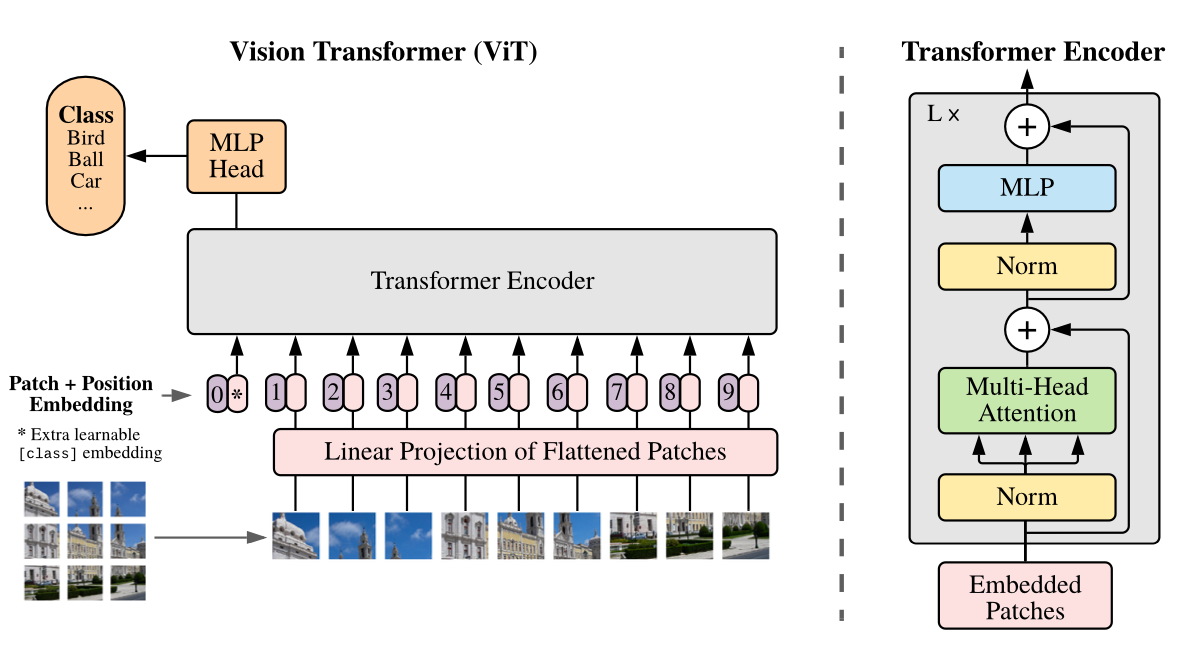
\includegraphics[width=0.8\textwidth]{img/1-section/Vision transformer.png} 
\end{center}

\end{frame}
\section{Architettura}


\begin{frame}
\frametitle{Split an image into fixed-size patches}

Naive application of self-attention to images would require that \textbf{each pixel attends to every other pixel}. With \textbf{quadratic cost} in the number of pixels, this does \textbf{not scale to realistic input sizes} (even with very small images)

\begin{center}
    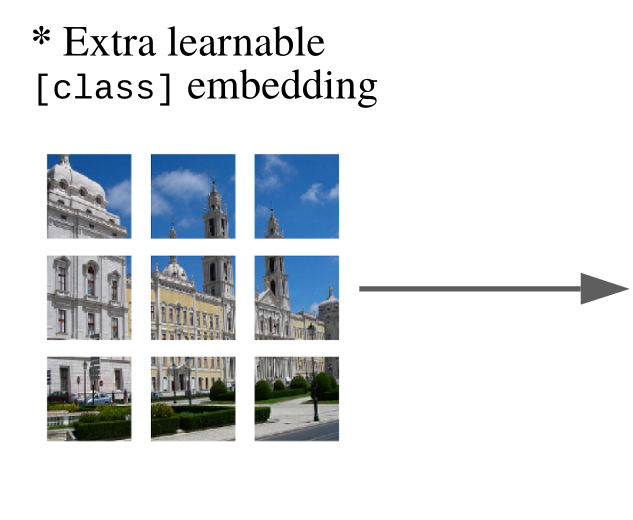
\includegraphics[width=0.5\textwidth]{img/2-section/Patching.png} 
\end{center}
\end{frame}

% \begin{frame}
% \frametitle{16x16 Patches}

%  ViT goes further to demonstrate that large scale pre-training makes \textbf{vanilla transformers competitive} with (or even better than) state-of-the-art CNNs. (Prior to this only 2x2 patches have been used)

% \begin{center}
%     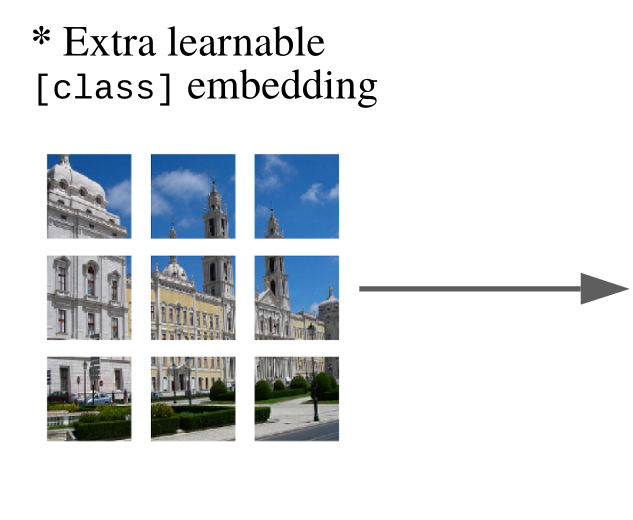
\includegraphics[width=0.5\textwidth]{img/2-section/Patching.png} 
% \end{center}
% \end{frame}


\begin{frame}
\frametitle{Position Embedding}

Positional Embedding provide information about the order of elements in a sequence, which is crucial for understanding \textbf{context}.

\vspace{0.5cm}

classification token token seves as as a global feature extractor that rappresents the entire image.

\begin{figure}[H]  % L'opzione [H] forza l'immagine a rimanere esattamente in quel punto nel testo
    \begin{center}
        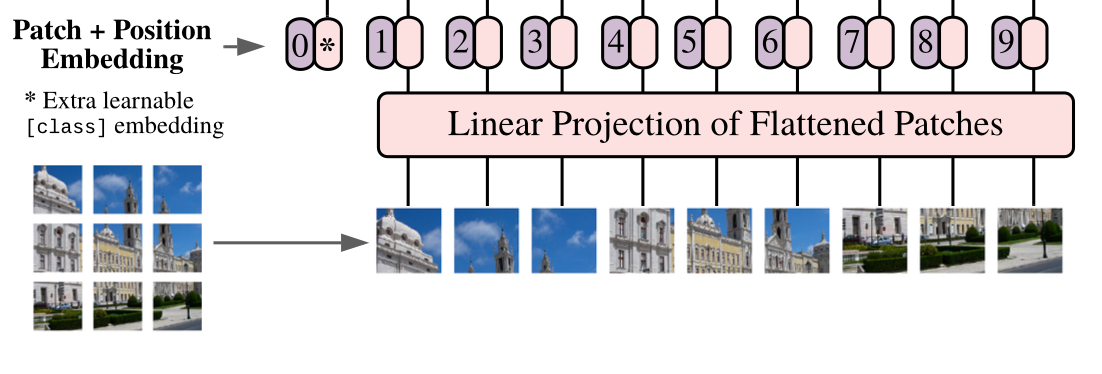
\includegraphics[width=0.8\textwidth]{img/2-section/Posizion enbedding.png}
        
    \end{center}
\end{figure}

\end{frame}

\begin{frame}
\frametitle{What type of Position Embedding?}

We can use a 1D or a 2D representation for Position Embedding

\begin{figure}
    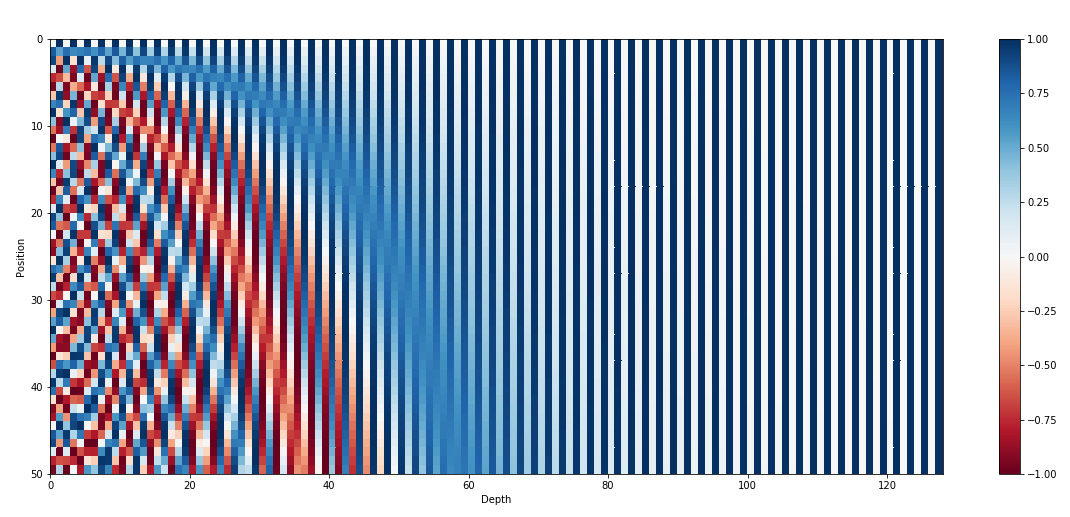
\includegraphics[width=0.8\textwidth]{img/2-section/positional_encoding.png} 
    \label{fig:Positional_encoding}
    \caption{Positional encoding matrix}
\end{figure}
\end{frame}

\begin{frame}
\frametitle{Transformer Encoding}


\begin{columns}
        \begin{column}{0.5\textwidth}
        Architecture of a Transformer:
            \begin{itemize}
            \item  Multi Head Attention
            \item Multi layer Perceptron (Feed Forward)
            \end{itemize}
        \end{column}
        \begin{column}{0.3\textwidth}
            \centering
            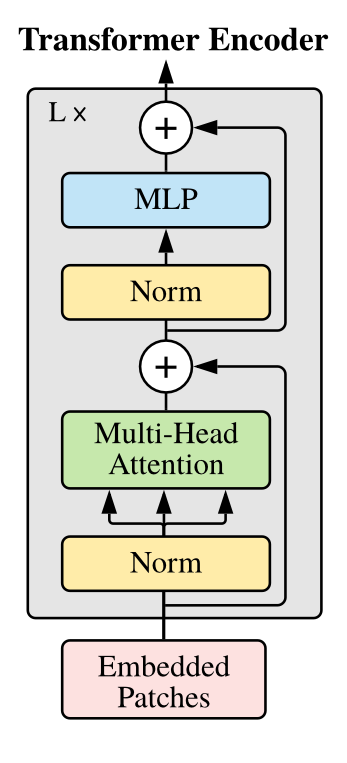
\includegraphics[width=\textwidth]{img/2-section/Transformer encoding.png}
        \end{column}
    \end{columns}


\end{frame}





\begin{frame}
\frametitle{Classification of the images}

After the last Transformer there is a MLP head that allow to classify each images.

\begin{center}
    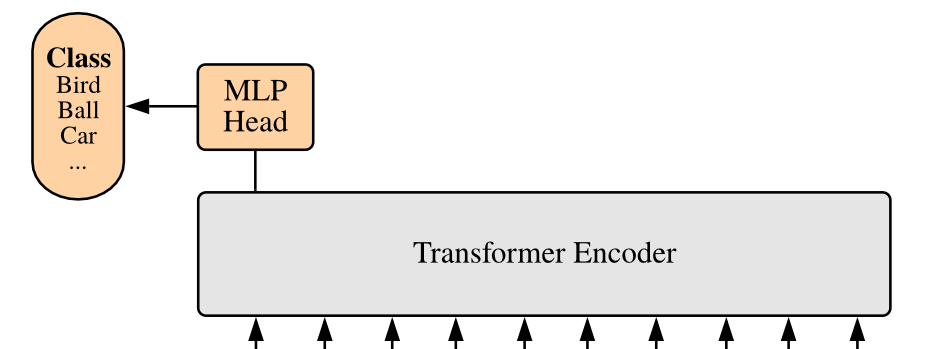
\includegraphics[width=0.8\textwidth]{img/2-section/Classification.png} 
\end{center}
\end{frame}
\section{Benchmark}

\begin{frame}
\frametitle{Dataset and models Different models}
Datasets:
\begin{itemize}
    \item ImageNet
    \item ImageNet Real (better labeling)
    \item JFT-300M with 18k classes and 303M high-resolution images
    \item CIFAR-10 6k 32x32 colour images in 10 classes, with 6000 images per class
    \item CIFAR-100 100 classes containing 600 images each
    \item Oxford-IIIT Pet 37 category 200 images for each class
\end{itemize}
\vspace{0.4cm}

Models:
\begin{center}
    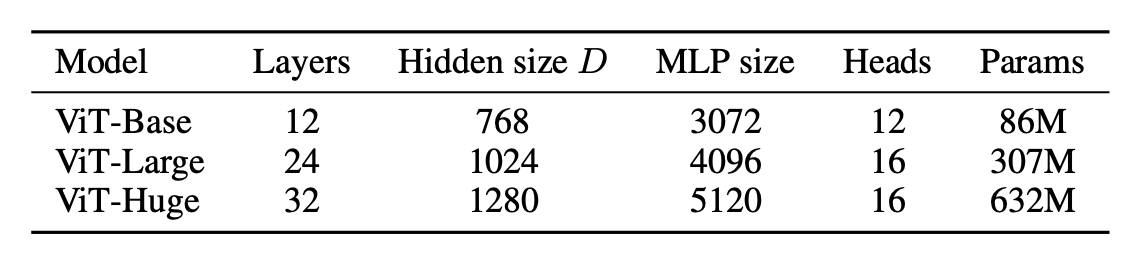
\includegraphics[width=0.8\textwidth]{img/3-section/Varianti VIT.png} 
\end{center}

\end{frame}

\begin{frame}
\frametitle{Results}
Comparison with state of the art on popular image classification benchmarks:
\begin{center}
    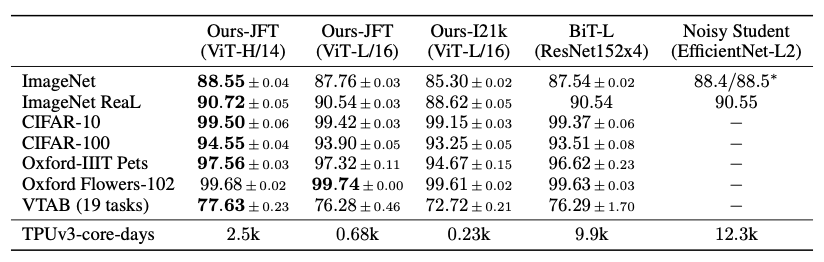
\includegraphics[width=1\textwidth]{img/3-section/Simple benchmark.png} 
\end{center}

Vision Transformer models pre-trained on the JFT-300M dataset outperform ResNet-based baselines on all datasets, while taking substantially less computational resources to pre-train

\end{frame}

\begin{frame}
\frametitle{Trained with different dataset}
Accuracy (\%) of Vision Transformer on various datasets when pretrained on ImageNet, ImageNet-21k or JFT300M
\begin{center}
    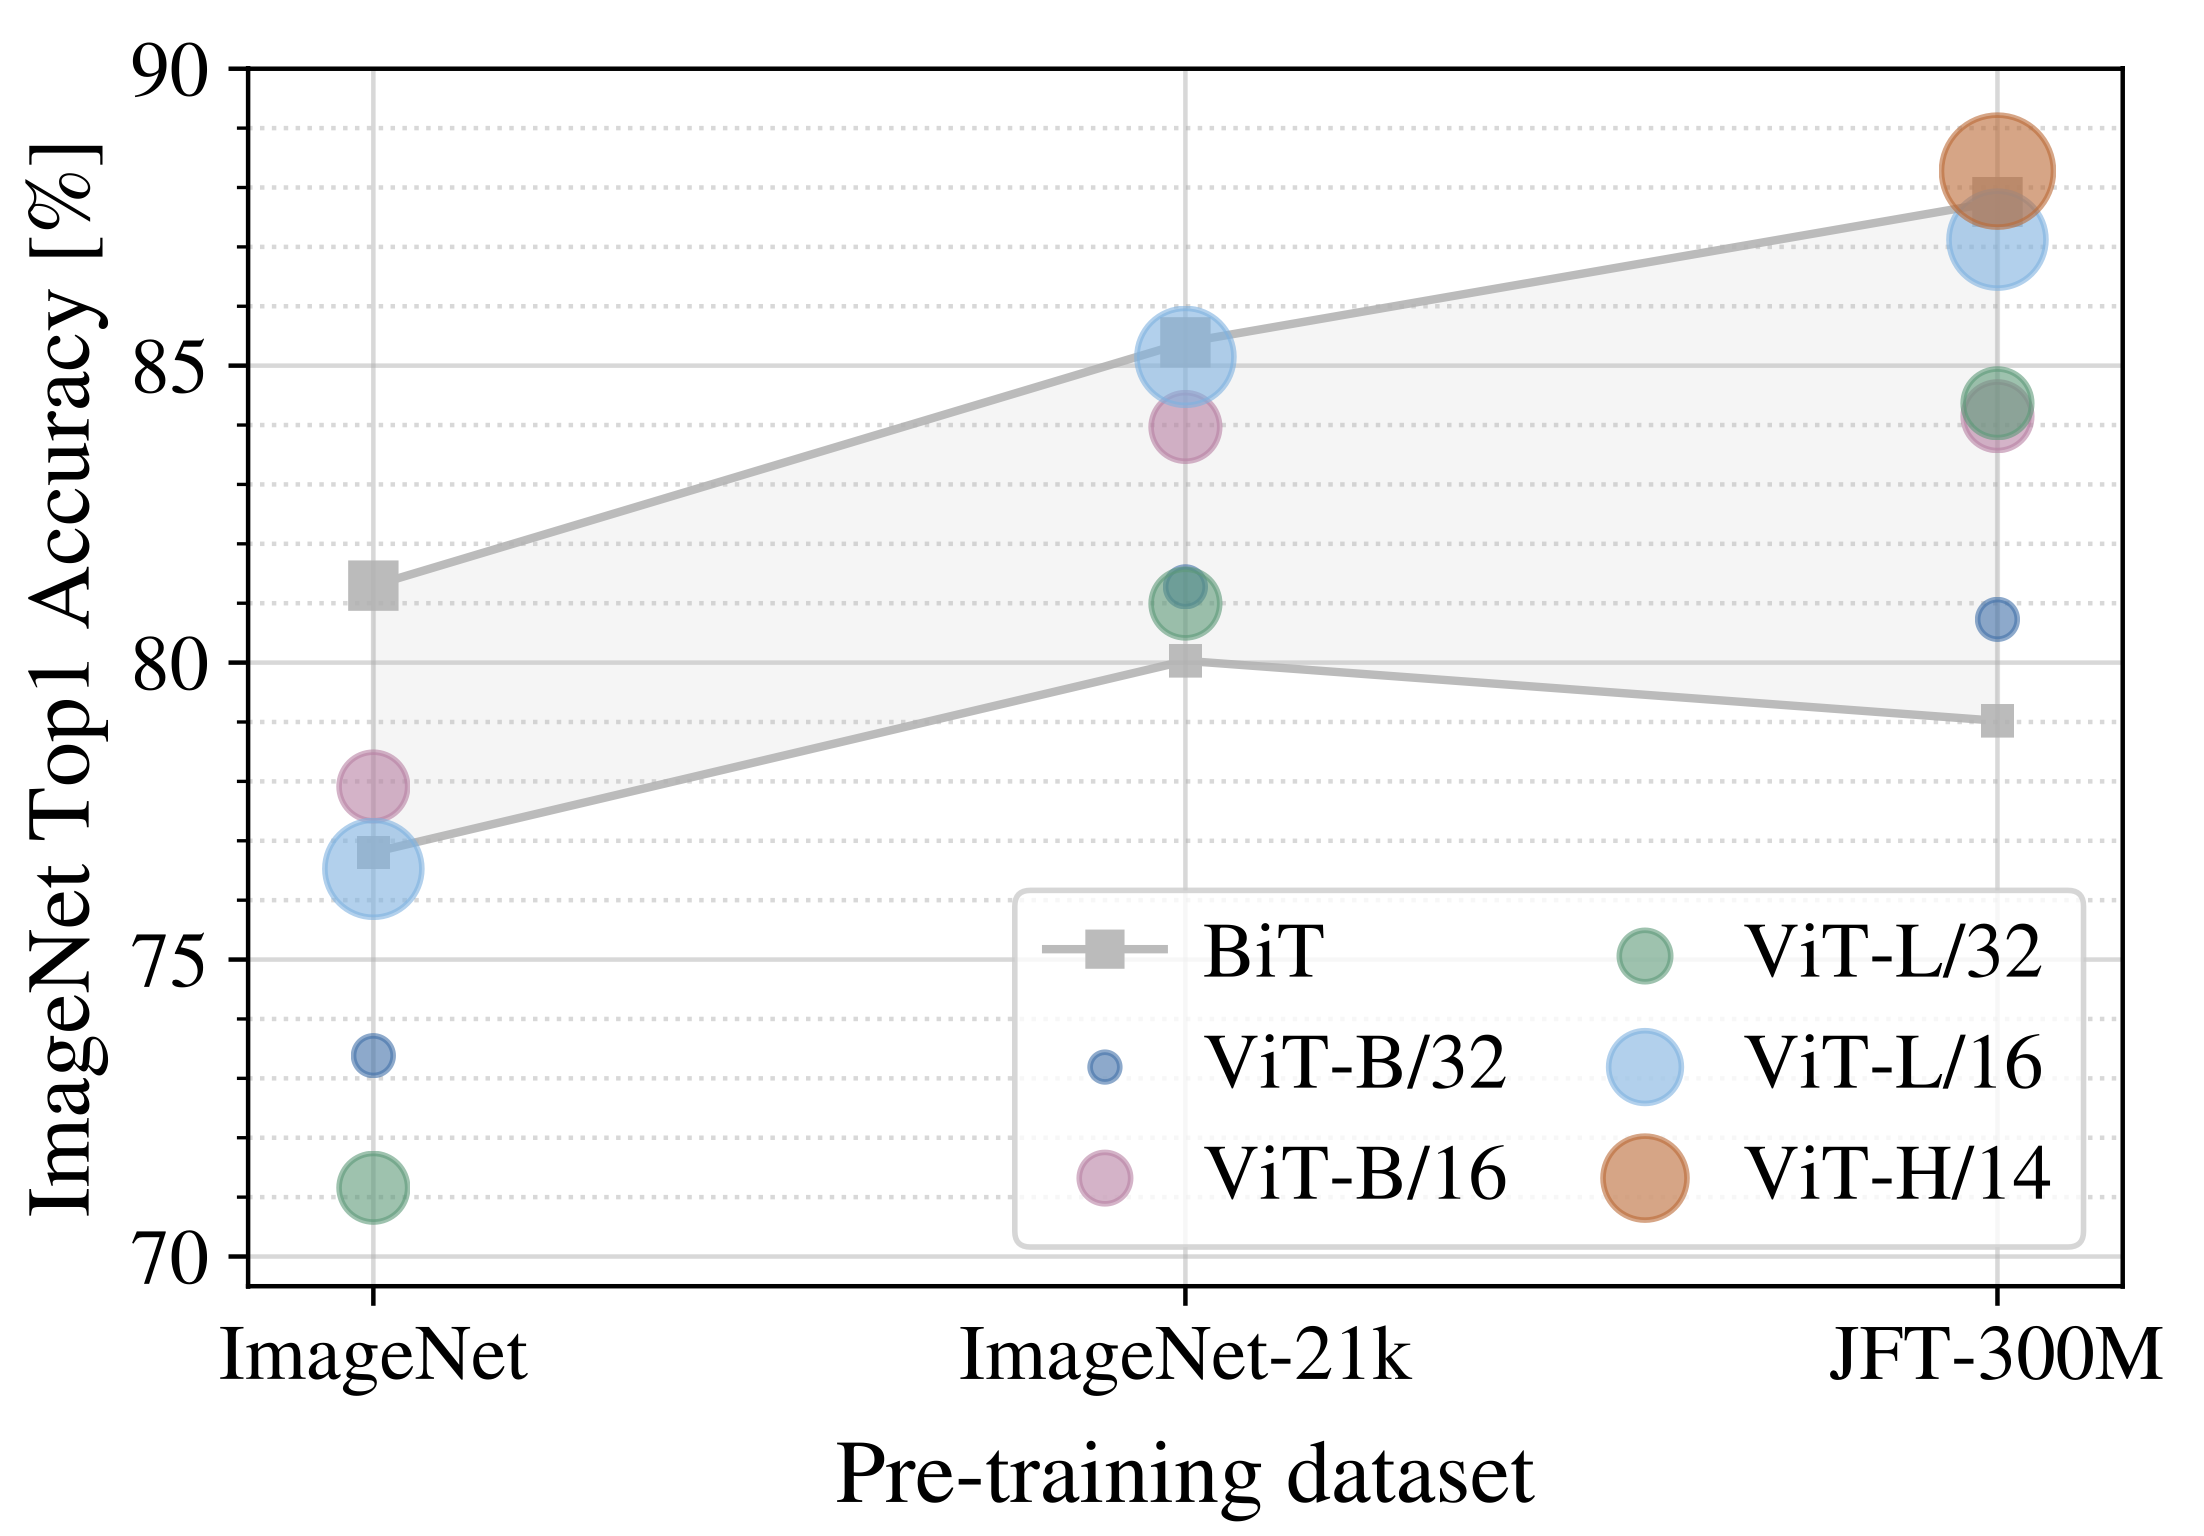
\includegraphics[width=0.5\textwidth]{img/3-section/Pretraining image.png} 
\end{center}
While large ViT models perform worse than BiT ResNets (shaded area) when pre-trained on small datasets, they \textbf{shine when pre-trained on larger datasets}. Similarly, larger ViT variants overtake smaller ones as the dataset grows.

\end{frame}


\begin{frame}
\frametitle{ConvNeXt by Facebook and Berkeley}
Reexamine the design space and push the limits of ConvNet potential, modernizing  standard ResNet towards a Transformer-like design, leading to the creation of ConvNeXt.

\begin{center}
    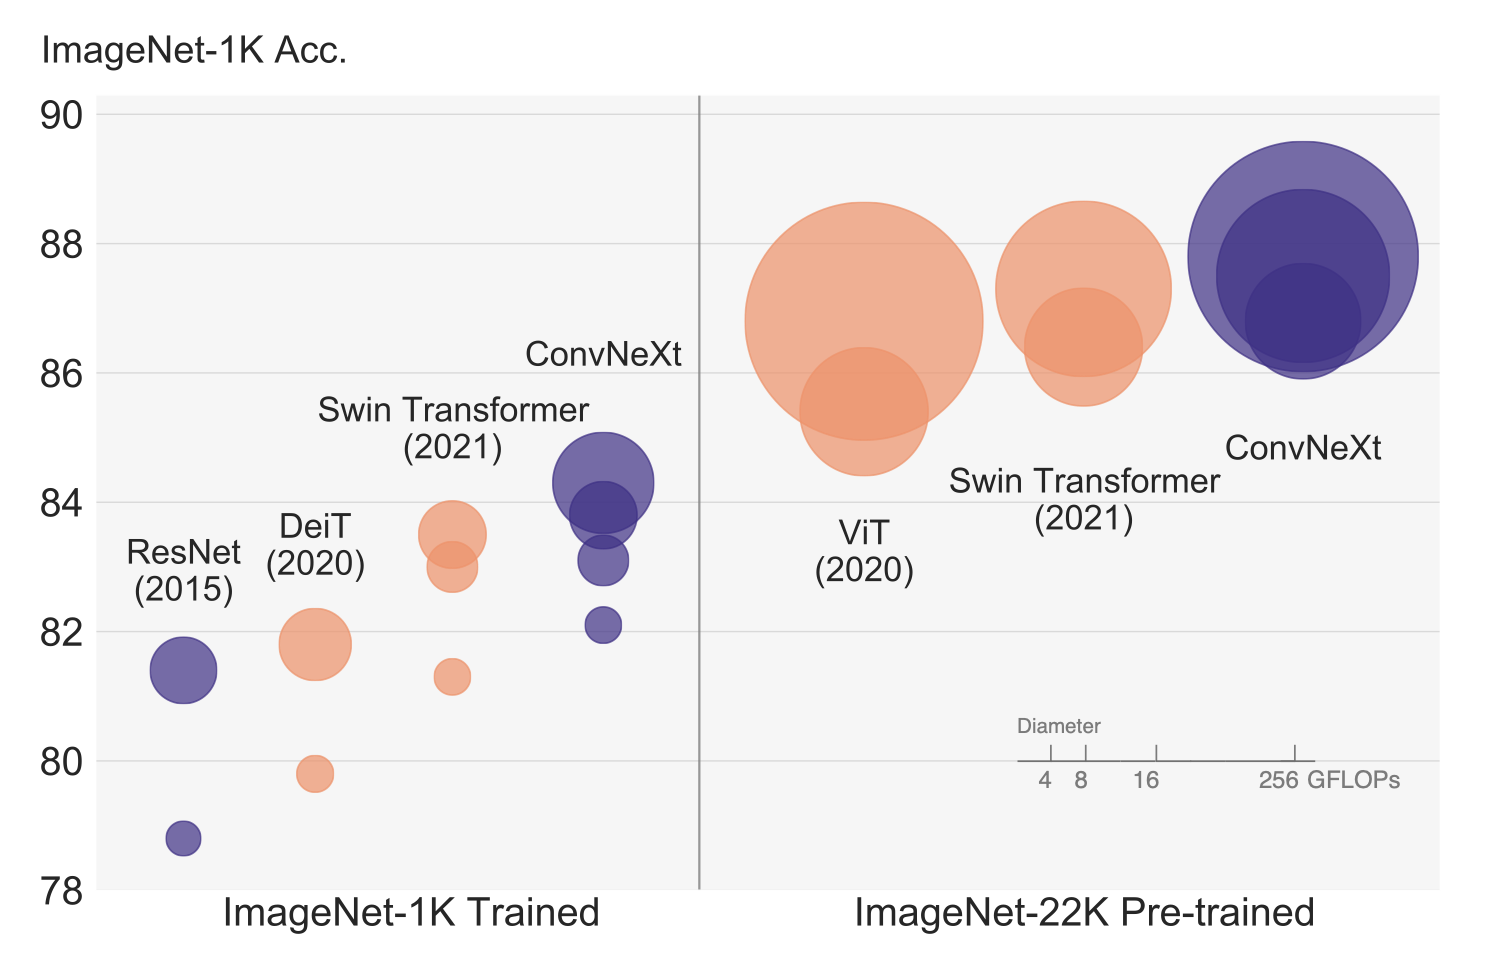
\includegraphics[width=0.7\textwidth]{img/3-section/ConvNext.png} 
\end{center}

\end{frame}

\begin{frame}
\frametitle{ConvNets Match Vision Transformers at Scale}
Google deepmind found out that ConvNets can match ViT at Scale

\vspace{0.5 cm}

\begin{center}
    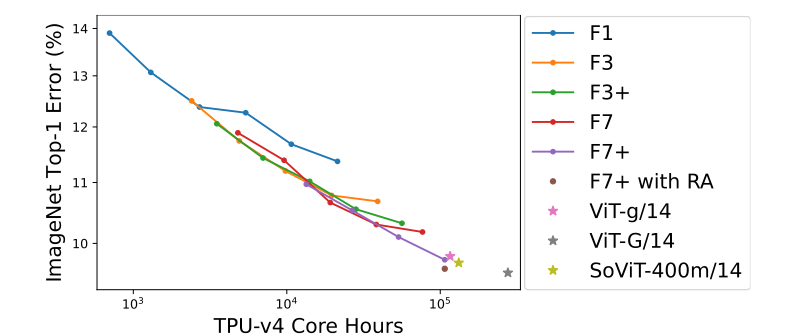
\includegraphics[width=0.7\textwidth]{img/3-section/log-log.png} 
\end{center}

Observed a log-log scaling law between held out loss (validation dataset) and compute budget.
\end{frame}

\begin{frame}
\frametitle{Key Observation, Google's point of view}

\vspace{0.5cm}
\begin{itemize}
    \item \textbf{Training Time:} The amount of computational resources and time dedicated to training the model
    \item \textbf{Dataset Quality and Size:} Access to large and diverse datasets, such as JFT-4B
\end{itemize}

\end{frame}




%----------------------------------------------------------------------------------------
%	CLOSING SLIDE
%----------------------------------------------------------------------------------------

\begin{frame}[plain] 
    \begin{center}
		{\Huge References:}
            
	\end{center}
	\begin{itemize}
    \item \href{https://arxiv.org/abs/1706.03762}{Attention Is All You Need}
    \item \href{https://arxiv.org/abs/2010.11929}{An Image is Worth 16x16 Words: Transformers for Image Recognition at Scale}
    \item \href{https://arxiv.org/pdf/2201.03545}{A ConvNet for the 2020s}
    \item \href{https://arxiv.org/abs/2310.16764}{ConvNets Match Vision Transformers at Scale}
\end{itemize}
\end{frame}


%----------------------------------------------------------------------------------------

\end{document} 